\def\year{2022}\relax
%File: formatting-instructions-latex-2022.tex
%release 2022.1
\documentclass[letterpaper]{article} % DO NOT CHANGE THIS
\usepackage{aaai22}  % DO NOT CHANGE THIS
\usepackage{times}  % DO NOT CHANGE THIS
\usepackage{helvet}  % DO NOT CHANGE THIS
\usepackage{courier}  % DO NOT CHANGE THIS
\usepackage[hyphens]{url}  % DO NOT CHANGE THIS
\usepackage{graphicx} % DO NOT CHANGE THIS
\urlstyle{rm} % DO NOT CHANGE THIS
\def\UrlFont{\rm}  % DO NOT CHANGE THIS
\usepackage{natbib}  % DO NOT CHANGE THIS AND DO NOT ADD ANY OPTIONS TO IT
\usepackage{caption} % DO NOT CHANGE THIS AND DO NOT ADD ANY OPTIONS TO IT
\DeclareCaptionStyle{ruled}{labelfont=normalfont,labelsep=colon,strut=off} % DO NOT CHANGE THIS
\frenchspacing  % DO NOT CHANGE THIS
\setlength{\pdfpagewidth}{8.5in}  % DO NOT CHANGE THIS
\setlength{\pdfpageheight}{11in}  % DO NOT CHANGE THIS
%
% These are recommended to typeset algorithms but not required. See the subsubsection on algorithms. Remove them if you don't have algorithms in your paper.
\usepackage{algorithm}
\usepackage{algpseudocode}
\usepackage{amssymb}
\usepackage{amsmath}

%
% These are are recommended to typeset listings but not required. See the subsubsection on listing. Remove this block if you don't have listings in your paper.
\usepackage{newfloat}
\usepackage{listings}
\lstset{%
	basicstyle={\footnotesize\ttfamily},% footnotesize acceptable for monospace
	numbers=left,numberstyle=\footnotesize,xleftmargin=2em,% show line numbers, remove this entire line if you don't want the numbers.
	aboveskip=0pt,belowskip=0pt,%
	showstringspaces=false,tabsize=2,breaklines=true}
\floatstyle{ruled}
\newfloat{listing}{tb}{lst}{}
\floatname{listing}{Listing}
%
%\nocopyright
%
% PDF Info Is REQUIRED.
% For /Title, write your title in Mixed Case.
% Don't use accents or commands. Retain the parentheses.
% For /Author, add all authors within the parentheses,
% separated by commas. No accents, special characters
% or commands are allowed.
% Keep the /TemplateVersion tag as is
\pdfinfo{
/Title (AAAI Press Formatting Instructions for Authors Using LaTeX -- A Guide)
/Author (AAAI Press Staff, Pater Patel Schneider, Sunil Issar, J. Scott Penberthy, George Ferguson, Hans Guesgen, Francisco Cruz, Marc Pujol-Gonzalez)
/TemplateVersion (2022.1)
}

% DISALLOWED PACKAGES
% \usepackage{authblk} -- This package is specifically forbidden
% \usepackage{balance} -- This package is specifically forbidden
% \usepackage{color (if used in text)
% \usepackage{CJK} -- This package is specifically forbidden
% \usepackage{float} -- This package is specifically forbidden
% \usepackage{flushend} -- This package is specifically forbidden
% \usepackage{fontenc} -- This package is specifically forbidden
% \usepackage{fullpage} -- This package is specifically forbidden
% \usepackage{geometry} -- This package is specifically forbidden
% \usepackage{grffile} -- This package is specifically forbidden
% \usepackage{hyperref} -- This package is specifically forbidden
% \usepackage{navigator} -- This package is specifically forbidden
% (or any other package that embeds links such as navigator or hyperref)
% \indentfirst} -- This package is specifically forbidden
% \layout} -- This package is specifically forbidden
% \multicol} -- This package is specifically forbidden
% \nameref} -- This package is specifically forbidden
% \usepackage{savetrees} -- This package is specifically forbidden
% \usepackage{setspace} -- This package is specifically forbidden
% \usepackage{stfloats} -- This package is specifically forbidden
% \usepackage{tabu} -- This package is specifically forbidden
% \usepackage{titlesec} -- This package is specifically forbidden
% \usepackage{tocbibind} -- This package is specifically forbidden
% \usepackage{ulem} -- This package is specifically forbidden
% \usepackage{wrapfig} -- This package is specifically forbidden
% DISALLOWED COMMANDS
% \nocopyright -- Your paper will not be published if you use this command
% \addtolength -- This command may not be used
% \balance -- This command may not be used
% \baselinestretch -- Your paper will not be published if you use this command
% \clearpage -- No page breaks of any kind may be used for the final version of your paper
% \columnsep -- This command may not be used
% \newpage -- No page breaks of any kind may be used for the final version of your paper
% \pagebreak -- No page breaks of any kind may be used for the final version of your paperr
% \pagestyle -- This command may not be used
% \tiny -- This is not an acceptable font size.
% \vspace{- -- No negative value may be used in proximity of a caption, figure, table, section, subsection, subsubsection, or reference
% \vskip{- -- No negative value may be used to alter spacing above or below a caption, figure, table, section, subsection, subsubsection, or reference

\setcounter{secnumdepth}{0} %May be changed to 1 or 2 if section numbers are desired.

% The file aaai22.sty is the style file for AAAI Press
% proceedings, working notes, and technical reports.
%

% Title

% Your title must be in mixed case, not sentence case.
% That means all verbs (including short verbs like be, is, using,and go),
% nouns, adverbs, adjectives should be capitalized, including both words in hyphenated terms, while
% articles, conjunctions, and prepositions are lower case unless they
% directly follow a colon or long dash
\title{Towards a robot partner reducing\\ ambiguities using perspective taking}
\author{
    %Authors
    % All authors must be in the same font size and format.
    Anthony Favier\textsuperscript{\rm 1,2},
    Shashank Shekhar\textsuperscript{\rm 1},
    Rachid Alami\textsuperscript{\rm 1,2}
}
\affiliations{
    %Afiliations
    \textsuperscript{\rm 1}LAAS-CNRS, Universite de Toulouse, CNRS, Toulouse, France\\
    \textsuperscript{\rm 2}{Artificial and Natural Intelligence Toulouse Institute (ANITI)}

    % email address must be in roman text type, not monospace or sans serif
    \{anthony.favier, sshekhar, rachid.alami\}@laas.fr
}

\begin{document}

%%%%% SYMBOLS DEFINITION %%%%%
\newcommand{\worldstates}{\mathcal{S}}
\newcommand{\worldstate}{s}
\newcommand{\fluent}[3]{\mathcal{F}^{#1#2}_{#3}}
\newcommand{\prop}{\varphi}
\newcommand{\allprops}{\Phi}
\newcommand{\predicate}{\mathcal{P}}
\newcommand{\predval}{v}
\newcommand{\agent}{\lambda}
\newcommand{\beliefs}{\mathcal{B}}
\newcommand{\human}{H}
\newcommand{\robot}{R}
\newcommand{\places}{\mathcal{P}}
\newcommand{\place}{p}
\newcommand{\unknown}{UnKw}
\newcommand{\known}{Kw}
\newcommand{\missedactions}{\mathcal{M}}
\newcommand{\loc}[1]{loc(#1)}
\newcommand{\obs}[1]{obs(#1)}
\newcommand{\dom}[1]{dom(#1)}
\newcommand{\observable}{\texttt{OBS}}
\newcommand{\inferrable}{\texttt{INF}}
%%%%%%%%%%%%%%%%%%%%%%%%%%%%%%

\maketitle

\begin{abstract}
\end{abstract}

\section{Introduction}
% what is known ? our understanding of the world
general context, towards robot partner. 

% what is unknown ? the gap we want to fill
% how and why ? your rational and purpose/hypothesis 

\clearpage
\section{Related Work / Background}

\begin{itemize}
    \item some refs from ICRA paper ? (Devin theory of mind) 
    \item human activity model, hierarchical HTN
    \item HATP general
    \item HATPEHDA (ICRA)
\end{itemize}

\section{Materials and Methods}
% what did you do ?

The work \cite{buisan:hal-03684211} already support collaborative task planning while maintaining distinct beliefs/knowledge for each agent. This work is itself an extension of HATP \cite{hatp?} having one search thread for a shared plan resulting in two coordinated plan streams. The last work HATPEHDA proposes a two threads search. Based on this work, we enhanced the task planner with a few concept linked to perspective taking and observability in order to reduce the ambiguities that may happen in a collaborative task. First we predict the situation assessment of an agent. On the other hand, we look for belief divergences that have a detrimental influence on the plan in order to fix them with communication. We also check observability of action execution to update beliefs with different types of effects.

Agents can have a shared goal but no shared plan. There is no plan negotiation between the agents, so the robot is only able to estimate what the human will do and plan its own actions according to that.

\subsection{HATPEHDA background/basis and definitions}

The main structure manipulated by our planner is the \textbf{agent}, more precisely two will be represented, the \textit{human} and the \textit{robot}. Each agent has their own \textbf{beliefs}, \textbf{action model}, \textbf{agenda}, \textbf{plan} and \textbf{triggers}. The planner has to use their action models and beliefs to decompose the tasks in their agenda into primitive tasks (actions) that are inserted in their plan. By doing so, it also has to update the beliefs of each agent and to model their reaction by executing the triggers. \cite{buisan:hal-03684211}.

The agents, robot and human, have each a distinct action model modeled with HTNs. The robot HTN starts with the goal given to the robot and describes how to decompose that abstract goal into several actions. The human HTN represents the anticipation by the robot of the human plan and possible actions in a given situation. Other formalism like POMPD or PDDL could be used to describe the agents' action models as soon as they provide the next possible actions of an agent in a given state. Especially the human one which is an estimation.

The planner has a goal creation mechanism, especially for the human, based on goal-directed or situation-directed task creation.

The planning algorithm is implemented as a search involving two threads: 1) the robot task-based plan search using the robot action model 2) the estimation of the human task-based plan search using the human action model.

While HTN-R corresponds to the controllable part  (from the robot point of view) of the (shared) plan, HTN-H represents the contigent part of the plan: the decisions and actions of the human. 

Hence, the obtained plan has two streams (one for the human and one of the robot) and is conditional. Alternatives correspond to human decision: choosing to act or not, making one (out of several choices).

As a result, HATP/EHDA allows to clearly separate what is planned for the robot and what the human can potentially do with respect to the task at hand. Besides, it allows to also:
\begin{itemize}
    \item deal with cases where the task is only given to the robot and not shared by the human
    \item manage the creation of a shared goal
    \item provide a mean to implement elicitation, by the robot, of decisions or reactions of the human
\end{itemize}
In our case the plan process starts:
\begin{itemize}
   \item with a goal given only to the robot: a task placed at the root of HTN-R (ex: Human asks the robot to achieve a goal)
   \item or with a shared goal: the same task is placed at the roots of  the two HTNs (ex: Human says to the robot: "Let us do X")
\end{itemize}

Situation-directed task creation in HTN-H allows to model (potential) reaction by the human to a situation created by after a given action of the robot. This can be used in the planner to elicit a reactiion of the human.

\subsection{Knowledge representation and observability definitions}

Our formalism is close to the SAS+ Formalism applied to HTN.  

\textbf{Places}: 
A place is an area defined a priori in the environment. Let $\places=\{ \place_i \}$ be the set of all defined places. Agents are always situated in a place or moving between them. Actions are always performed in a place. (Most?) State variables are associated to a place.

\textbf{Observation of an action execution}: 
For simplification purposes we define the notion of co-presence. Two agents located in a same place are said to be co-present.
Based on that, we assume that the execution of an action performed by an agent $\agent$ has been observed by all agents that were co-present with $\agent$ either before or after the action. The co-presence is checked both before and after to cover navigation actions.
(As future work a more elaborated formula could be used to evaluate the observation of an action execution, for instance using geometrical reasoning.)

\textbf{Word state}: 
% Let $\worldstates$ be the set of all possible world states, any world state is defined by a set of fluents i.e. $\forall\worldstate\in\worldstates, \worldstate=\{ \fluent{\worldstate}{}{}{} \}$.
Let $\worldstates$ be the set of all possible world states. World states are defined by a same set of fluents. Each world state is fully described by the value of all fluents at a given time i.e. $\forall\worldstate\in\worldstates, \worldstate=\{ \fluent{\worldstate}{}{}{} \}$.

\textbf{Fluent}: 
A fluent $\fluent{\worldstate}{}{}{}$ is a multi-valued state variable associated to a finite domain $Dom(\fluent{\worldstate}{}{}{})$ partially describing the state of the world at a given time.

e.g. Considering the following fluent $\fluent{\worldstate}{}{temp\_water}{}$, if initially the water is hot then $\fluent{\worldstate_0}{}{temp\_water}{}=hot$.



\textbf{Belief divergence}: 
We note $\fluent{\worldstate}{,\agent}{}{}$ a fluent evaluated in the perspective of an agent $\agent$. Thus, for a given real state of the world $\worldstate\in\worldstates$, the robot and the human can have different values for the same fluent. We call such mismatch a belief divergence.

e.g. $(\fluent{\worldstate_0}{,\robot}{temp\_water}{}=hot) \neq (\fluent{\worldstate_0}{,\human}{temp\_water}{}=cold)$

\textbf{Two distinct Beliefs}: 
We call beliefs of an agent $\agent$, noted $\beliefs_\agent$, the belief state in which this agent thinks the world is in, i.e. the set of all fluents evaluated in their perspective at a given time: $\beliefs_\agent=\{ \fluent{\worldstate}{,\agent}{}{} \}$. It is important to note that we use two distinct belief states during the planning process. On one hand, we consider the beliefs of the robot $\beliefs_\robot$ which are obtained through perception and effects of robot actions and decisions. As we consider the planner as being part of the robot, we assume that $\beliefs_\robot$ is the ground truth estimation for the planner. On the other hand, we consider the human's belief state $\beliefs_\human$ which is only estimated by the robot by doing some perspective-taking reasoning during the planning process.

\textbf{Observability of fluents}:
Each fluent is associated to a place $\place \in \places$ through the relation $\loc{ \fluent{\worldstate}{}{}{} }=\place$. These relations help to describe the world state by expressing where the fluents are effective and observable. These relations can be dynamic if the fluent describes a property linked to a moving entity (agents, movable objects). However, currently the location of a fluent has to be updated manually in the domain if it is dynamic (we should go for an "entity-based" description of the world state to automatically update).

The observability of each fluent is qualified through the relation $\obs{ \fluent{\worldstate}{}{}{} } \in \{ \observable, \inferable \}$. 
% The first value $\observable$ means that the fluent is observable. More details on how this property is used will be given in the \textit{Situation Assessment} part but keep in mind that a fluent is observed by an agent only if it is observable and if that agent is in the place associated to the fluent. 
The first value $\observable$ means that the fluent is observable. A fluent is observed by an agent only if it is observable and if that agent is in the place associated to the fluent (co-present with fluent?). This property is used in the \textit{Situation Assessment} process.
The other value $\inferable$ qualifies inferable fluents. A fluent is inferable if its value isn't observable but can be inferred by attending an action affecting that fluent. For instance, by observing someone adding salt to a dish we infer that there is now salt in the dish, although the salt in the dish isn't observable. It means that without attending the action execution it's impossible to tell if there salt just by looking at it. Thus, we consider that when an action affects inferable fluents only the co-present agents gets their beliefs updated. We later refer to actions affecting inferable fluents as actions with some inferable effects.

\textbf{Situation Assessment}:
The idea is to predict the situation assessment of an agent and update their beliefs according to what they can see in their current place. The situation assessment is executed after every action execution. When executed, each agent update their beliefs with the ground truth value of every observed fluents, i.e. for every observable fluents ($\obs{ \fluent{\worldstate}{}{}{} } = \observable$) located in their place ($\loc{\fluent{\worldstate}{}{}{}} = \fluent{\worldstate}{}{at}{,\agent}$), we have $\fluent{\worldstate}{,\agent}{}{} \gets \fluent{\worldstate}{}{}{}$. Note that since we use the ground truth world state, which is actually the robot beliefs, this situation assessment is only effective for the human. 

With our symbolic place-based model of observability we assume that the observabilty of each fluent is constant and defined initially by the scenario. Note that even with this simplified model we can cover scenarios where an object is suddenly not observable by defining a dedicated place for this obstructed state. For instance, if an object is put inside a cupboard (move object to place \textit{inside\_cupboard}), an agent will be able to observe the object only if they open the cupboard (move agent to place \textit{inside\_cupboard}) or if they get the object out (move object to same place as the agent).

\textbf{Beliefs update after action [draft]}: 
When an agent performs an action, the beliefs are updated differently according to if the agent is the robot or the human. 
About the robot beliefs updates, especially when the robot doesn't observe a human action. Using explicit values of state variables, it makes no sense for the robot to know that it doesn't know something.
For now we assume that if the human has to do something that is planned and not observable by the robot it should be quite simple. Thus, we suppose it's ok to apply all effects instantly.
Thus, when the human is performing an action, the acting agent beliefs $\beliefs_\human$ are updated as well as the robot ones $\beliefs_\robot$, with all effects.
When the robot is performing an action, again the acting agent beliefs, $\beliefs_\robot$, are updated. Then, only if the human and the robot are co-present $\beliefs_\human$ gets updated with the inferable effects of the robot action. The human beliefs will be updated with all other observable effects thanks to the situation assessment.

\textbf{Relevant belief divergences checking}:
We want to detect if a belief divergence influences the plan of the human, i.e. if when using the human beliefs containing belief divergences induces different human actions than the ones expected using the ground truth beliefs. If so, the belief divergences are qualified as relevant. Indeed, a belief divergence can wrongly affect the applicability of a human action, its cost and its effects. 
Any difference in the human plan makes it either not applicable in reality, more expensive or with undesired effects. There are some rare cases of belief divergences inducing a different plan still applicable, with a similar cost and no undesired effects. But for now we omit these cases and we consider relevant belief divergences as always detrimental.

To check if there are some relevant belief divergences we proceed as follows. When refining the human agenda to estimate their next possible actions, we first use the human beliefs $\beliefs_H$. The process is repeated but considering the robot beliefs $\beliefs_R$ (ground truth). The two obtained refinements are then compared to check if they are the same. Two refinements are considered to be the same if they respectively have the same decompositions, i.e. if, in both refinements, each decomposition respectively has the same type, subtasks and if their actions have the same applicability, cost and effects. If the two refinements are not the same we consider that there are relevant belief divergences to align, but we don't know which ones yet.

\textbf{Identify the relevant divergences and communicate}: 
Once the presence of relevant belief divergences has been confirmed they have to be identified. All divergences between $\mathcal{B}_R$ and $\mathcal{B}_H$ are first computed. Then the divergence's corrections are simulated one after another (i.e. $ \fluent{\worldstate}{,\human}{i}{} \gets \fluent{\worldstate}{,\robot}{i}{}$) and the human agenda is refined again in order to compare the new refinement with the one previously obtained with $\beliefs_\robot$. We keep simulating combination of divergence corrections in a breadth-first (search) manner until the refinements are the same, which means that all the relevant divergences have been identified. In the worst case, the last combination corresponds to all divergences being corrected, which means $\beliefs_\human$ and $\beliefs_\robot$ are now the same. Thus the obtained refinements will necessarily be the same which guarantees the ending of our algorithm. After having identified the divergences to correct in order to obtain the same refinements, the corresponding communication action is inserted in the robot's plan to inform the human about their relevant belief divergences and to correct them.
    
Communication actions are supposed to be instantaneous (0 time step to execute), to be able to correct sevaral divergences at the same time and for now they are inserted right before the detected erroneous human action. (A more complex reasoning could be added to identify the optimal place to insert the communicaton action in the plan). 

\subsection{Algorithm}

The refinement of the HTNs is mostly done thanks to the function $refineAgenda()$. This function keeps refining the agenda of an agent in a given state until reaching a not done primitive task at the first spot. It returns a refinement which is list of decomposition, one for each applicable methods. Each decomposition is a list of the obtained subtasks which starts with a not done primitive task. The second parameter the function $refineAgenda$ can be used to specify with which beliefs the refinement has to be done. 

The returned refinement in \ref{alg:ap_ref_all} contains the subtasks obtained through the refinement of the agenda after a potential belief alignement, application of the actions, situation assessment and triggers.

\begin{algorithm}
\caption{Get applied refinement ALL}\label{alg:ap_ref_all}
\begin{algorithmic}
\Require $h\_name$: human name, $r\_name$: robot name, $ags$: all agents

\State $ref \gets refAgenda(ags, ag\_name)$

\State $ref\_r \gets refAgenda(ags, r\_name)$ \Comment{H only}
\If{$relevantDivergences(ref, ref\_r)$} \Comment{H only}
    \State $alignBeliefsWithComAction()$
    \State $ref \gets refAgenda(aligned\_ags, h\_name)$
\EndIf

\For{$decomp$ in $refinement$}

    \State $result \gets applyOperator(dec, ag\_name)$ 
    \If{$notApplicable(result)$}
        \State \texttt{add wait, idle or end}
    \Else
        \State $applyOperator(dec, r\_name)$ \Comment{H only}
        \State $applyInferableEff(dec, h\_name)$ \Comment{R only}
        \State $humanSituationAssessment()$
        \State $checkTriggers()$
        \State $updateDecomp(decomp)$
    \EndIf
\EndFor

\State \Return ref

\end{algorithmic}
\end{algorithm}

\textbf{Choice to reduce ambiguities}:
In the case of a shared goal, let's assume that the human didn't observe the robot performing an action with only inferable effects, so when coming back the human has no way to tell if the action has been done just by looking at the scene. Then three cases can occur : 1) The human considers that the robot didn't perform the action, thus the human will try to perform it again, 2) The human considers that the robot performed the action so the plan execution continues, 3) the human prefers to directly ask the robot if it performed the action. 
Humans are rational so they will rarely blindly act without at least asking the state of the shared plan. However, whatever case we are in an ambiguity will remain for the human and we are able to predict it. Thus we decide to proactively reduce the ambiguity by communicating about their belief divergences or the missed actions. This communication might seem optional in some situations but having a plan without ambiguities in the context of a shared goal is often much better than a plan with less steps but where agent aren't sure about what they have to do. Communication help to compel the human actions.

\section{Results}
% what results did you get ?

Present example : Probably cooking example turning fire (situation assessment) and adding salt (relevant divergence). Show plan without our contribution. Then show what we obtain with our contribution.



Think about other configuration of the same scenario for other cases ? Here prevent action with undesired effects. Should find also applicability and cost.

Quantitative: We can randomize or use all combination of initial state : pasta location, starting agent, initial agent location, (initial belief divergence ?). Make statistics on applicability of plans with and withou contribution 

Qualitative :

For these examples, the world state is composed of the following fluents :\\
- $\fluent{\worldstate}{}{salt}{} \equiv salt\_added(s)\in\{true, false\}$\\
- $\fluent{\worldstate}{}{fire}{} \equiv pot\_fire\_on(s)\in\{true, false\}$\\
- $\fluent{\worldstate}{}{at}{, \{\robot,\human,pasta\} } \equiv at(e, s)\in \{place_1, place_2\}$
% , e \in \{ \robot, \human, pasta \}$

\begin{figure}
    \centering
    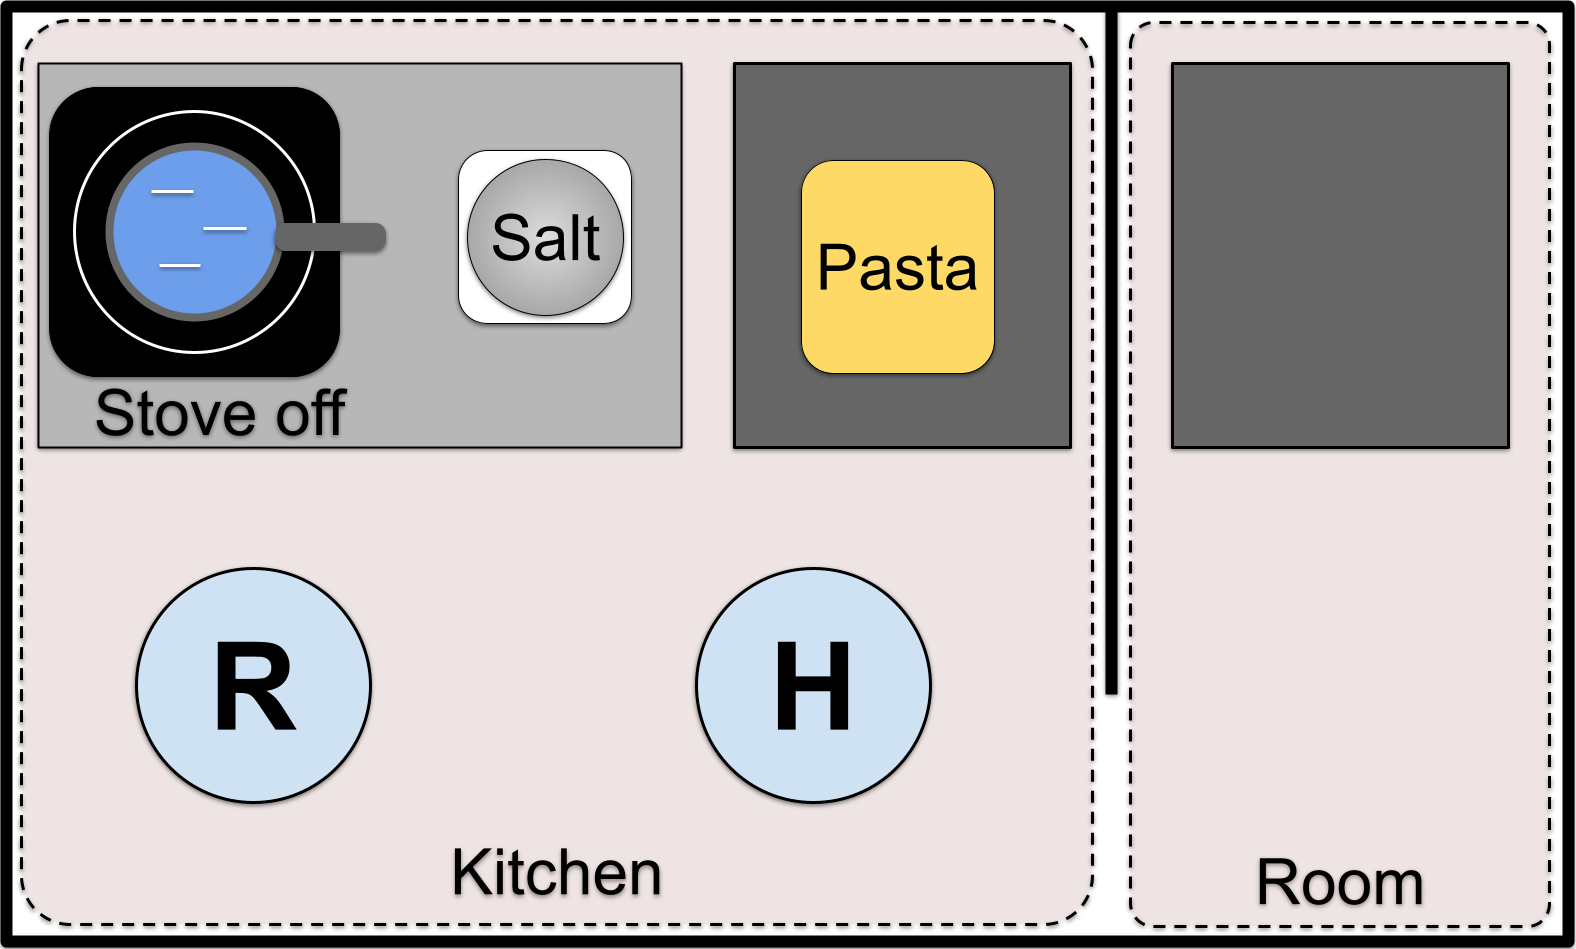
\includegraphics[width=0.8\linewidth]{figures/scene.png}
    \caption{Scene cooking}
    \label{fig:scene}
\end{figure}

Task description in HTN depicted in Fig.~\ref{fig:htn}

\begin{figure}
    \centering
    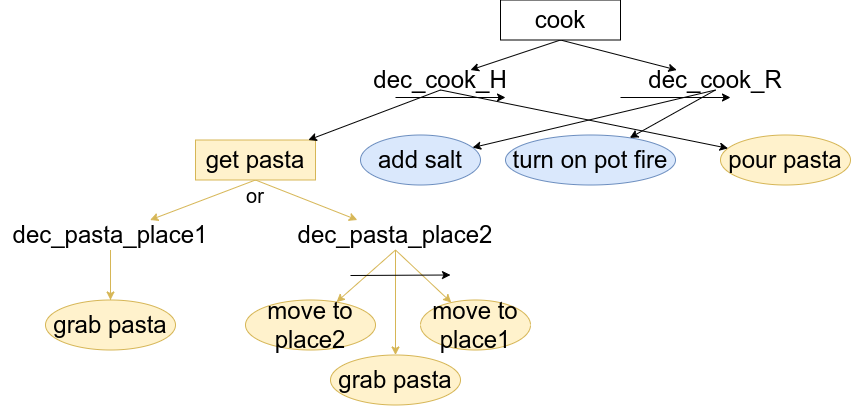
\includegraphics[width=\linewidth]{figures/htn.png}
    \caption{HTN, cook task description}
    \label{fig:htn}
\end{figure}

\begin{figure*}
    \centering
    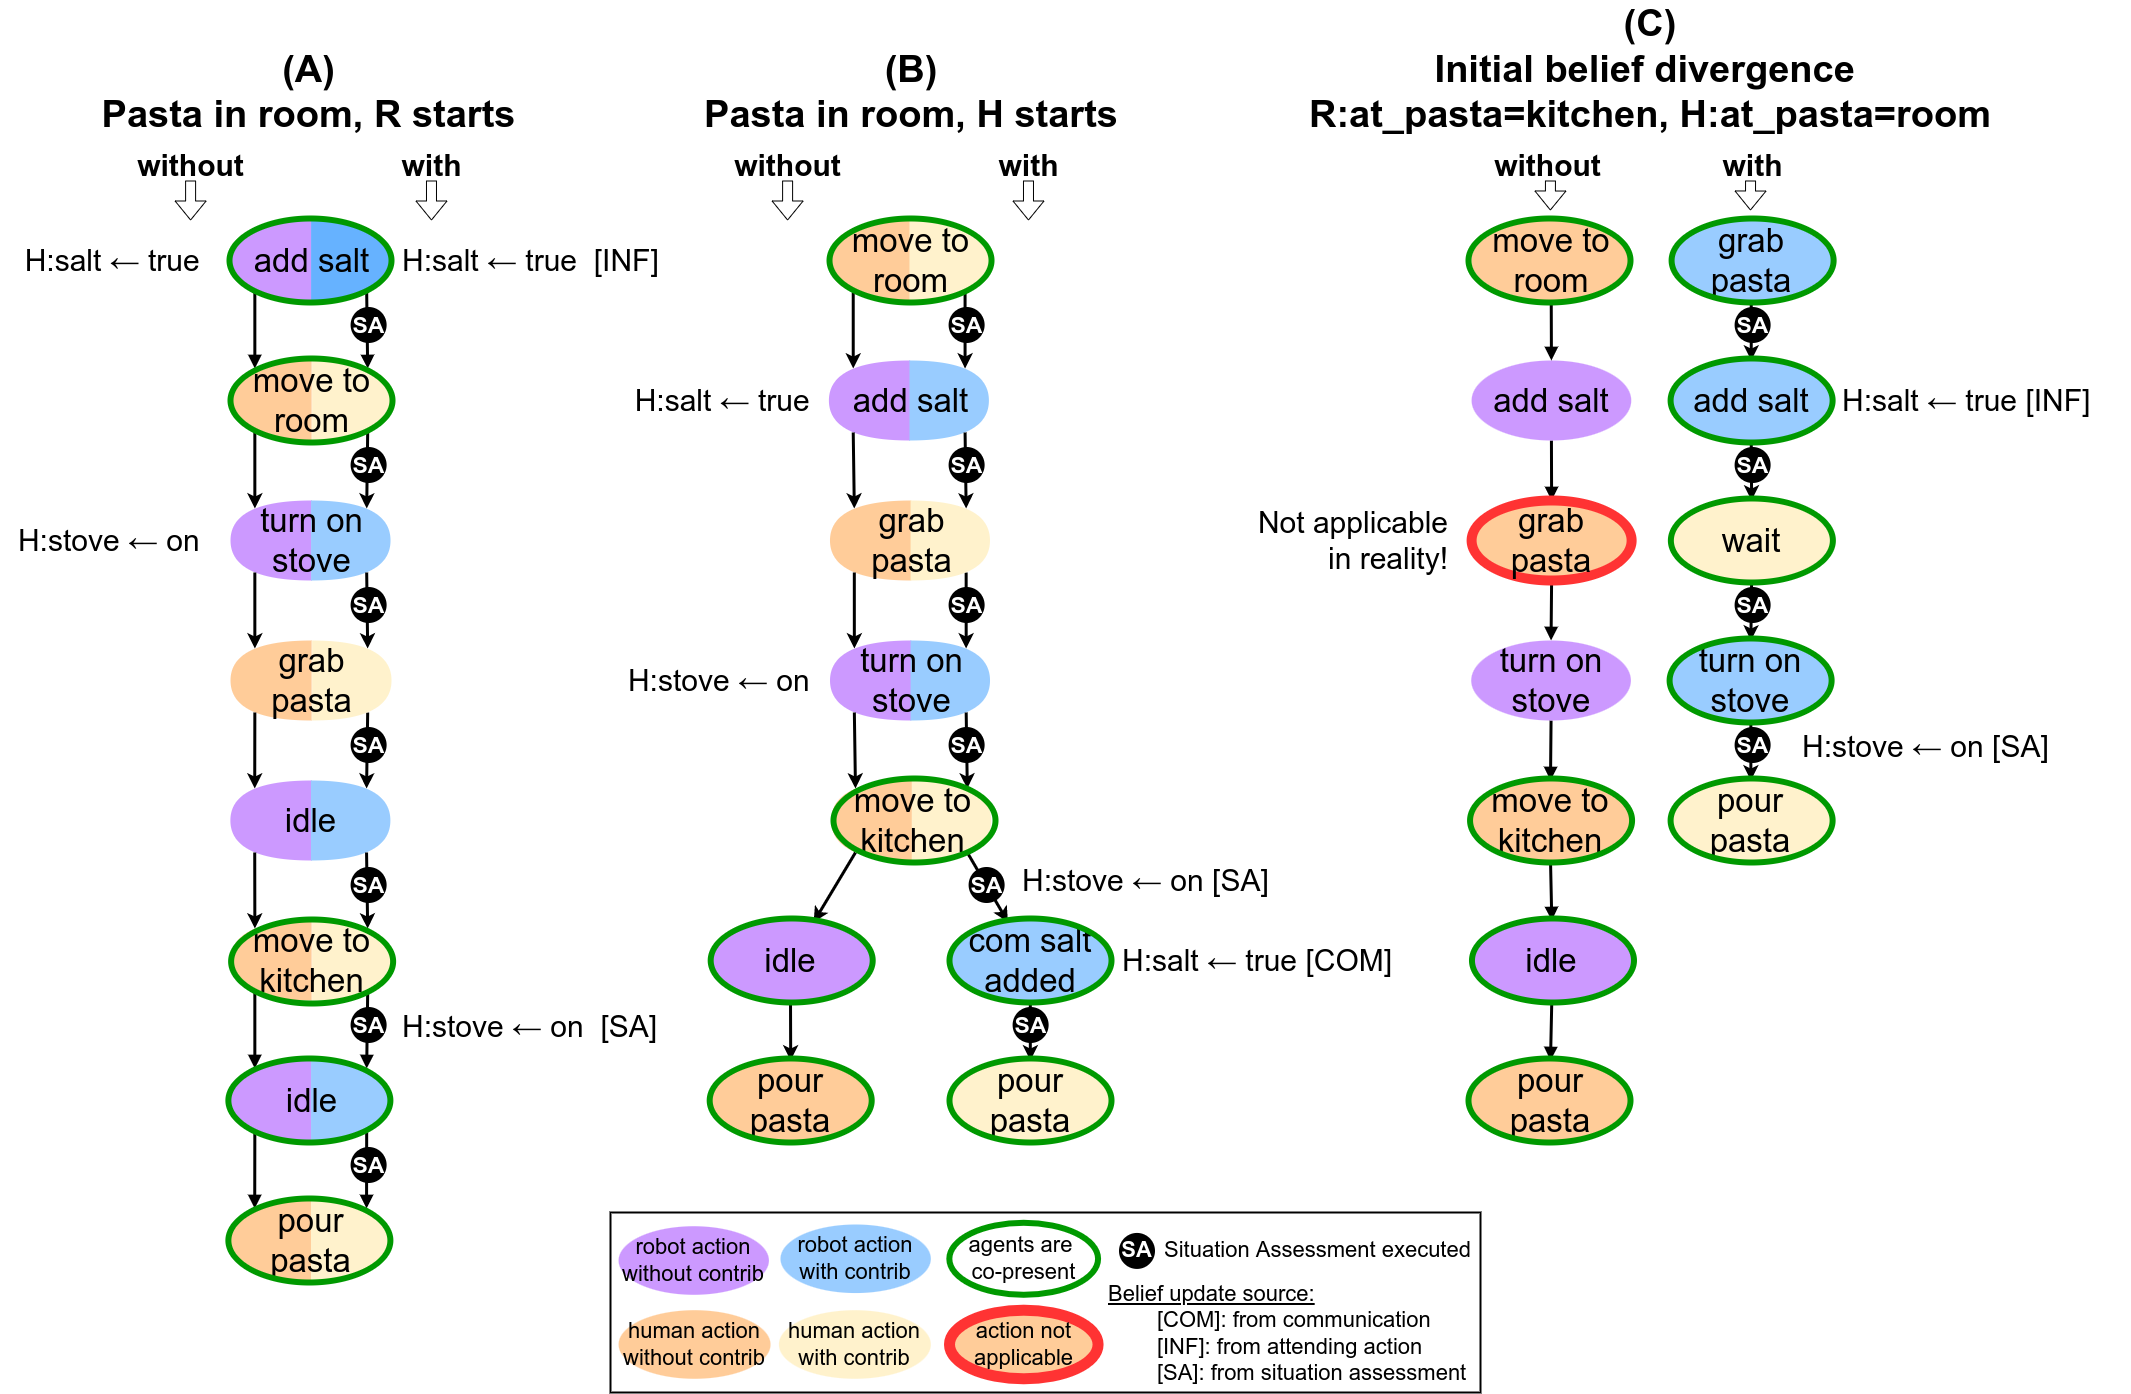
\includegraphics[width=\linewidth]{figures/example_cook.png}
    \caption{Caption}
    \label{fig:scenarios}
\end{figure*}







Scenarios:
\begin{itemize}
    \item \textbf{pasta in same place}
        normal execution
    
    \item \textbf{pasta in another place, R starts}
        w/o: Agents are omniscient, H knows instantly about the effects of R actions even without observing the actions
        w/: H sees salt action and assess the fire on action when coming back. Thus no com required, same plan than w/o but beliefs have been updated differently
        
    \item \textbf{pasta in another place, H starts}
        w/o: Agents omniscient again, H knows about all R actions instantly
        \subitem w/: R predicts H will miss both actions but will be able to assess the pot fire action execution when back in place1 but can't be sure about salt action. Decides to com to remove ambiguitiy
    
    \item \textbf{initial belief divergence on pasta location(R:place1 H:place2). The robot brought the pasta closer before the human comes}
        \subitem w/o: Plan isn't actually applicable with ground truth knowledge (grab pasta, no pasta here)
        \subitem w/: Relevant belief divergence detected. R com to correct the relevant divergence and make H plan applicable
    
    
\end{itemize}

\section{Discussion}
% how do the results fill the gap ?

Point out ambiguities (created both by the lack of situation assessment and belief alignment) in the plans without contribution. Then, explain how we removed them. 

\section{Conclusion}
% what does this mean for us going forward ?

FUTURE WORK:
\begin{itemize}
    \item A more elaborated formula for observability than co-presence. Using geometrical reasoning with a physic simulator.
    \item Use an entity-based world description to be able to automatically update the $\loc{\fluent{\worldstate}{}{}{}}$
\end{itemize}

\bibliography{bib.bib}

\end{document}
